\documentclass[11pt,a4paper,oneside]{article}
% input the config file
\usepackage[a4paper,margin=0.5in]{geometry}
\usepackage[separate-uncertainty=true,range-phrase=--]{siunitx}
\usepackage[utf8]{inputenc}
\usepackage[T1]{fontenc}
\usepackage{mathtools}
\usepackage{amsfonts}
\usepackage{amsthm}
\usepackage{booktabs}
\usepackage{thmtools}
\usepackage{amssymb}
\usepackage{graphicx}
\usepackage{enumitem}
\usepackage{tabularx} 
\usepackage[sfdefault]{roboto}
\usepackage[bibstyle=numeric,citestyle=alphabetic,natbib=false,backend=biber,sorting=ynt,sortcites=true,autocite=plain,hyperref=true,backref=true,maxbibnames=15,minbibnames=10,maxnames=15,minnames=10]{biblatex}
\usepackage{csquotes}
\usepackage{fancyhdr}
\usepackage{titlesec}
\usepackage{lipsum}
\usepackage{multicol}
\usepackage{flafter}
\usepackage{wrapfig}
\usepackage[usenames,dvipsnames]{xcolor}
\usepackage{pagecolor}
\usepackage{tcolorbox}
\usepackage[pdftex,hyperfootnotes=false,pdfpagelabels]{hyperref}
\usepackage[capitalise,noabbrev]{cleveref}
% no indentation for paragraphs, instead add more vertical spacing
\usepackage[skip=1ex,indent=0em]{parskip}

% make links/urls in bold
% https://tex.stackexchange.com/questions/47468/how-to-make-url-bold
\def\UrlFont{\bfseries}
% https://tex.stackexchange.com/questions/351650/make-all-href-text-bold
\LetLtxMacro\oldhref\href
\RenewDocumentCommand{\href}{o m m}{%
  \IfValueTF{#1}
    {\oldhref[#1]{#2}{\bfseries #3}}
    {\oldhref{#2}{\bfseries #3}}%
}
\addbibresource{bibliography.bib}

\titleformat{name=\section}{\huge\bfseries\sffamily\color{BlueViolet}}{\thesection}{.5em}{}
\renewcommand{\headrulewidth}{0pt}

% https://tex.stackexchange.com/a/17101/11281
% for logos in the same line as text in title page
\newcommand{\vcenteredinclude}[1]{\begingroup
  \setbox0=\hbox{\includegraphics[keepaspectratio,height=4ex]{#1}}%
\parbox{\wd0}{\box0}\endgroup}

% For section authors
\newcommand{\sectionauthor}[1]{\begingroup
{\color{Blue}\textbf{\large #1\\}}\rule{\textwidth}{0.4pt}\endgroup}

% Make submitter names bold in references
% The bibliography entry must include another field for this
% https://tex.stackexchange.com/a/304968/11281
\renewcommand*{\mkbibnamegiven}[1]{%
  \ifitemannotation{highlight}
    {\textbf{#1}}
    {#1}}

\renewcommand*{\mkbibnamefamily}[1]{%
  \ifitemannotation{highlight}
    {\textbf{#1}}
    {#1}}


%\definecolor{ocnspagecolor}{RGB}{255, 241, 213}
\definecolor{ocnspagecolor}{RGB}{255, 250, 241}


% document begins
\begin{document}

\pagestyle{plain}
\newgeometry{top=0mm,bottom=0mm,left=0mm,right=0mm}
\begin{titlepage}
  \quad{}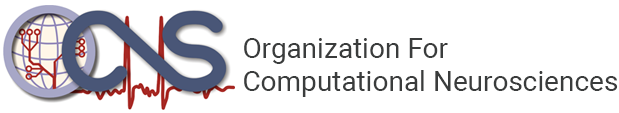
\includegraphics[width=0.8\textwidth,keepaspectratio]{./images/ocns-logo}
  \begin{tcolorbox}[colback=gray, colframe=black, width=\textwidth, boxrule=0.5mm, leftrule=0mm, rightrule=0mm,sharp corners=all]
  \vspace{1ex}
  \textbf{\textcolor{white}{Member Newsletter\quad{}|\quad{}October 2024\quad{}|\quad{}Volume 8 No 2}}
  \vspace{1ex}
  \end{tcolorbox}
  \topskip0pt
  \vspace{-1.35ex}
  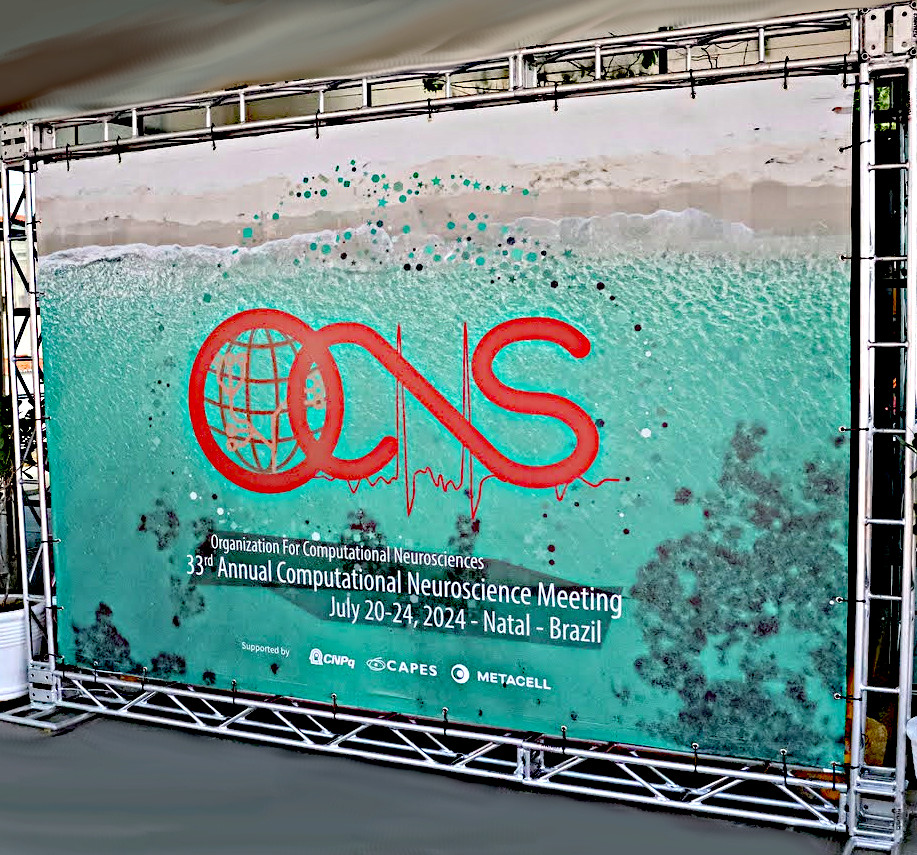
\includegraphics[width=\linewidth,keepaspectratio]{./images/ocns-newsletter-cover}
  \vspace{4ex}

  \vspace{1ex}
  \begin{center}
    \href{https://mastodon.social/@OCNS}{\vcenteredinclude{./images/Mastodon_Logotype_(Simple).svg}}~
    \href{https://twitter.com/cnsorg}{\vcenteredinclude{./images/X-logo}}~
    \href{https://www.facebook.com/CNSorg/}{\vcenteredinclude{./images/Facebook_icon_2013.svg}}~
    \textbf{\Large @CNSOrg}
    \hspace{1.2cm}\href{https://www.instagram.com/cns_ocns/}{\vcenteredinclude{./images/cropped-black-instagram-logo}}~
    \textbf{\Large @cns\_ocns}
    \hspace{1.2cm}\href{https://www.youtube.com/@ocns9820}{\vcenteredinclude{./images/youtube-logo}}~
    \textbf{\Large @ocns9820}
    \hspace{1.2cm}\href{https://www.linkedin.com/company/organization-for-computational-neurosciences/}{\vcenteredinclude{./images/LinkendIn}}~
    \textbf{\Large @OCNS}\vspace*{\fill}
  \end{center}
\end{titlepage}

\restoregeometry

\clearpage

\pagestyle{fancy}
\fancyhead{}
\fancyfoot{}
\fancyfoot[L]{Volume 8 No 2}
\fancyfoot[C]{OCNS Newsletter}
\fancyfoot[R]{Page \thepage}

\clearpage
\section*{Message from the President}%
\sectionauthor{Thomas Nowotny, Professor of Informatics, University of Sussex, UK}
\begin{wrapfigure}{l}{0.2\textwidth}
  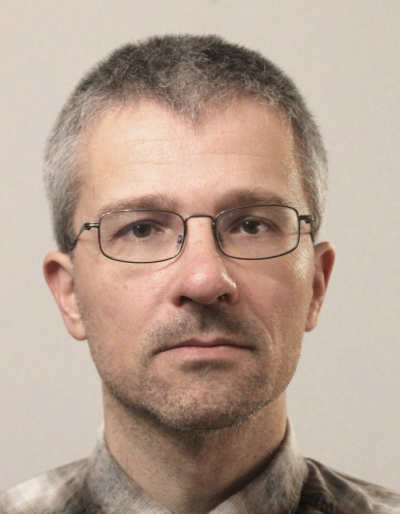
\includegraphics[width=0.2\textwidth]{images/Thomas}
\end{wrapfigure}

\lipsum[1-3]

\clearpage
\section*{CNS*2024 Natal: Report from Local Organizer}%
\sectionauthor{Cesar}
\begin{wrapfigure}{l}{0.2\textwidth}
  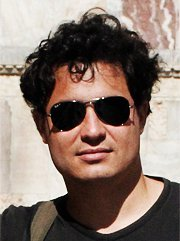
\includegraphics[width=0.2\textwidth]{images/Cesar}
\end{wrapfigure}

\lipsum[1-3]

\clearpage
\section*{CNS*2024 Natal: Messages from Volunteers}%
\sectionauthor{Messages from volunteers at CNS*2024 Natal}
\lipsum[1-3]

\clearpage
\section*{CNS*2024 Natal: Pictures}%
\sectionauthor{  }
See all the pictures online here \url{https://photos.app.goo.gl/YtpTN6ui4ap6P8Bz6}.

\clearpage
\clearpage
\clearpage
\section*{CNS*2024 Natal: From the Program Committee Chair}%
\sectionauthor{Julie Haas, Lehigh University, USA}
\begin{wrapfigure}{l}{0.2\textwidth}
  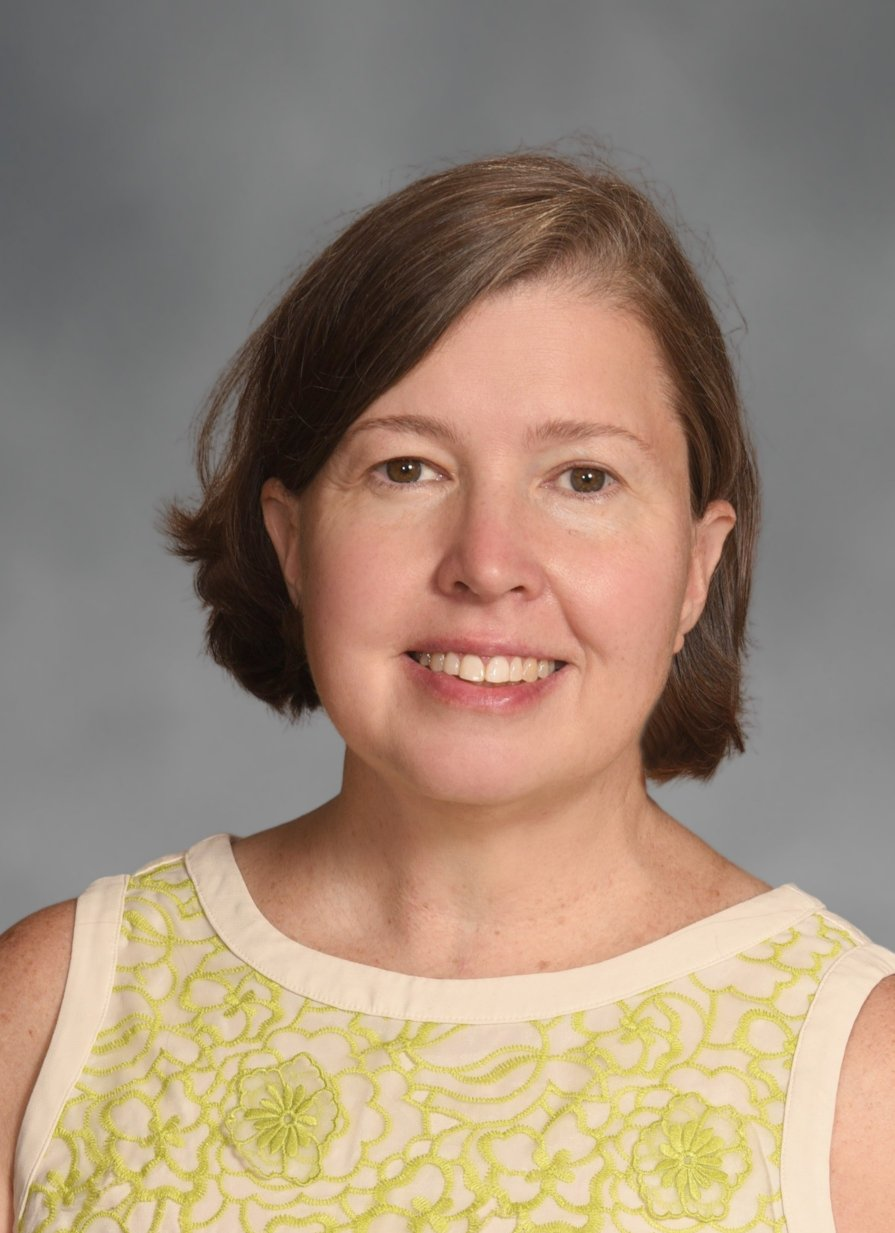
\includegraphics[width=0.2\textwidth]{images/Haas}
\end{wrapfigure}

\noindent{}Many thanks to Axel Hutt (Deputy Chair), Sang Wan Lee, Ian Stevenson and Nassi Papoutsi for their service, and extend a warm welcome to Andre Peterson, Masanori Shimono, Yunliang Zang and Arezoo Alizadeh.
We're currently working on selecting keynotes for CNS*2025 Florence, and look forward to a robust round of abstract reviewing in spring.

\clearpage

\section*{CNS*2024 Natal: Travel Awards}%
\sectionauthor{Travel Awards Chair:\ Michelle Moerel, Maastricht Centre for Systems Biology, Netherlands}
\begin{wrapfigure}{l}{0.2\textwidth}
  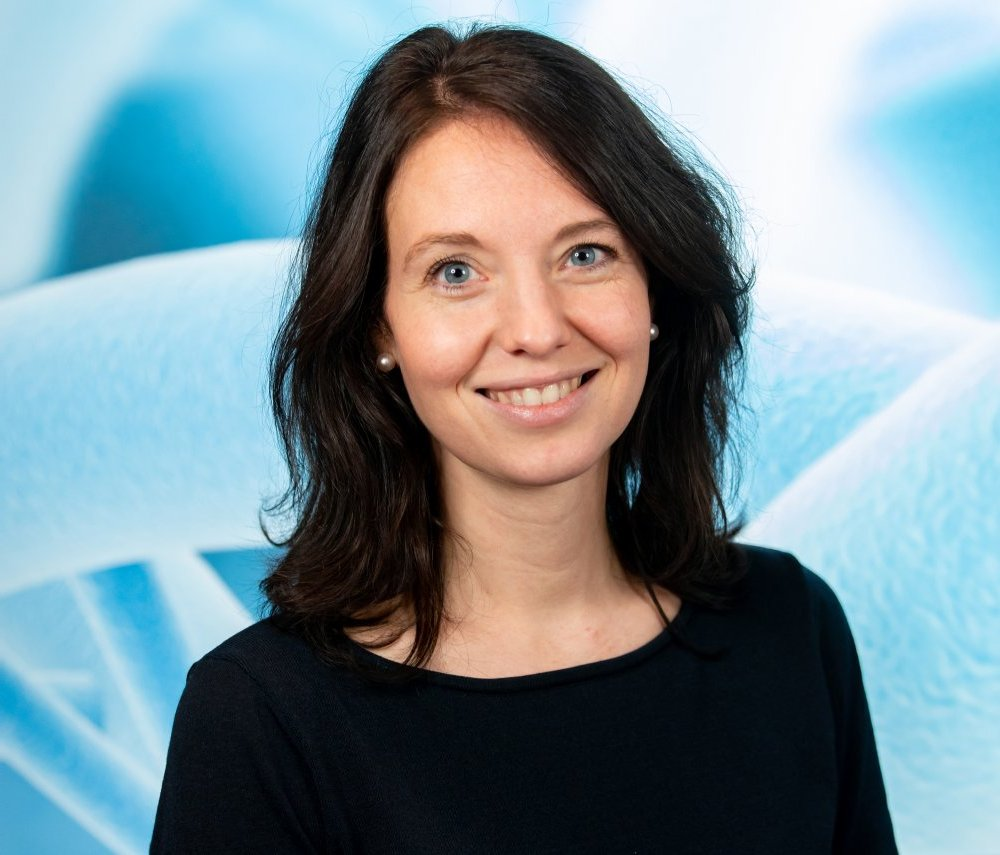
\includegraphics[width=0.2\textwidth]{images/Moerel}
\end{wrapfigure}

\noindent{}A limited number of merit based travel awards, given based on review of summaries by the program committee, are available to presenting students and postdocs who are OCNS members. Women and members of other historically marginalized communities in Science, Technology, Engineering, and Mathematics are particularly encouraged to apply.
Applications for travel grants are to be submitted during the abstract submission process at the annual OCNS conference.

This year's travel awards were competitive, with many more excellent applicants than available funds.
We were pleased to award 19 travel grants to participants from all over the world:

\begin{multicols}{2}
    \begin{itemize}
      \item Flavio Rusch (Brazil)
      \item Cecilia Jarne (Argentina)
      \item Paolo Protachevicz (Brazil)
      \item Fernando Fagundes Ferreira (Brazil)
      \item Pamela Alejandra Illescas Maldonado (Chile)
      \item Lavinia Mitiko Takarabe (Brazil)
      \item Forough Habibollahi Saatlou (Australia)
      \item Fabio Pioggio (Italy)
      \item Richard Gast (USA)
      \item Alexandra Chatzikalymniou (USA)
      \item Ankur Sinha (UK)
      \item Christopher Earl (USA)
      \item Anaelle De Worm (Belgium)
      \item Ferdinand Tixidre (France)
      \item Camille Mazzara (Italy)
      \item Lindsay Stolting (USA)
      \item Elnaz Nemati (Australia)
      \item Dirk Goldschmitt (UK)
      \item Eleonora Bernasconi (UK)
    \end{itemize}
\end{multicols}
\vspace{2ex}
\centerline{\rule{0.5\textwidth}{0.4pt}}
\vspace{4ex}
\noindent{}{\color{Blue}\textbf{\large Quotes from a few travel awardees:\\}}

\noindent{}\textbf{Flavio Rusch (Brazil)}
\begin{displayquote}
Attending CNS*2024 was an invaluable experience in my career as a physicist working in computational neuroscience. It provided me the opportunity to present my research to leading figures in the field, engage in discussions, and expand my network of collaborations. I am deeply grateful to OCNS for the travel award, as it made this opportunity possible.
\end{displayquote}

\vspace{2ex}
\noindent{}\textbf{Fabio Poggio (Italy)}
\begin{displayquote}
Receiving the travel award to attend CNS 2024 was a significant opportunity to engage with the latest advances in computational neuroscience and to exchange ideas with leading experts in the field. This experience has significantly enriched my research and professional growth, and I highly recommend it to anyone passionate about computational neuroscience.
\end{displayquote}
\clearpage
\noindent{}\textbf{Pamela Illescas (Chile)}
\begin{displayquote}
CNS 2024 in Natal was a wonderful experience to learn and share my doctoral thesis on networks with neuron-astrocyte interactions, which allowed
me to receive feedback from other researchers and opportunities for collaboration. This meeting was my first international computational neuroscience conference, and it was possible thanks to the CNS travel award. I am very grateful for this opportunity because it allows me to contribute to computational neuroscience in my country and internationally.
\end{displayquote}

\vspace{2ex}
\noindent{}\textbf{Cecilia Jarne, (Argentina)}
\begin{displayquote}
Attending CNS 2024 was an invaluable experience that allowed me to share our work on Hidden Markov Models (HMMs) software through the tutorial sessions offered at the conference. It also allowed me to present a poster on my ongoing research in predicting brain age, fostering meaningful discussions. I am very grateful for the travel award, which made this enriching experience possible.
\end{displayquote}




\clearpage
\section*{CNS*2024 Natal: Feedback form Summary}%
\sectionauthor{Tatiana Kameneva, Swinburne University of Technology, Australia (Registrations Chair)}
\begin{wrapfigure}{l}{0.2\textwidth}
  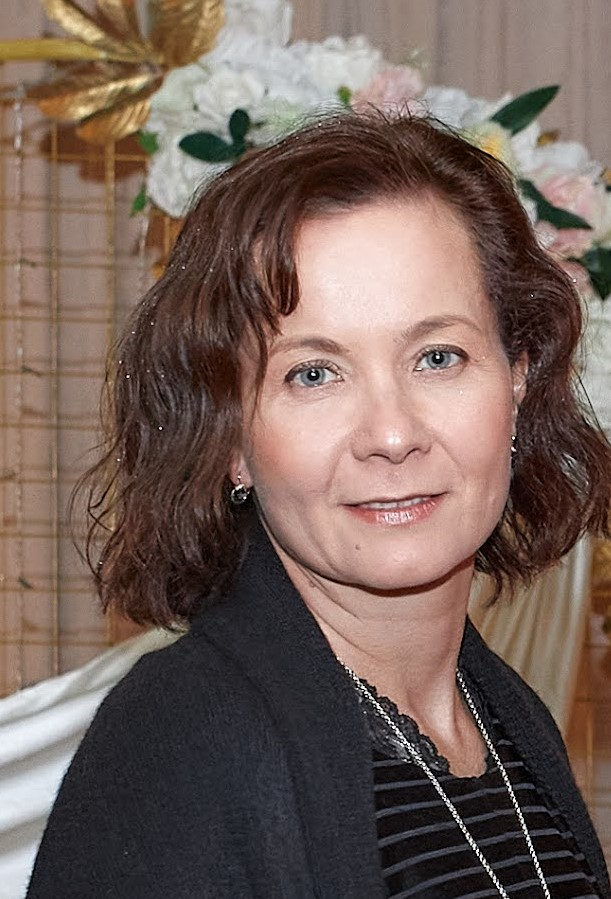
\includegraphics[width=0.2\textwidth]{images/Kameneva}
\end{wrapfigure}

\noindent{}We received 42 responses on the Participant Feedback Survey distributed at the end of CNS*2024.
Overall, the feedback has been positive. The data is presented in \cref{fig:cns2024-summary} above, with 5 being the highest rating.

Most people have enjoyed the venue: 71\% gave 4 or 5 rating in this category (\cref{fig:cns2024-summary} A).
Attendees commented highly on the quality of the keynote speakers: 55\% gave the highest (5) rating in this category (\cref{fig:cns2024-summary} B).
The common theme was a commendation to the local organizers for catering, efficiency, and airport pickup; while the AV, staff English proficiency, and the small space allocated for posters received mostly negative comments.

Tutorials had mixed reviews: 10\% of the attendees submitted the rating less than average satisfaction (1 or 2), while most people, 42\%, gave the rating 4 (\cref{fig:cns2024-summary} C). No comments were provided.

The attendance at the workshops varied.
Some workshops received very high praise; 80\% of people gave ratings 4 or 5, with comments such as \enquote{very interesting topics}, \enquote{amazing}, \enquote{excellent session} (\cref{fig:cns2024-summary} D).
While other workshops left attendees dissatisfied, with suggestions to reduce the number of parallel sessions to boost the attendance.

Overall, 79\% attendees enjoyed oral presentations and gave the ratings 4 or 5, while 21\% rated the presentation as satisfactory (3) or below (2), \cref{fig:cns2024-summary} E.
Positive comments included \enquote{OCNS is superb in supporting young scientist's careers}.
Suggestions for improvements included more talks on data-driven, deep learning-based approaches.
We thank everybody for their feedback that will be taken into account when organizing CNS*2025.

\begin{figure}[!h]
  \centering
  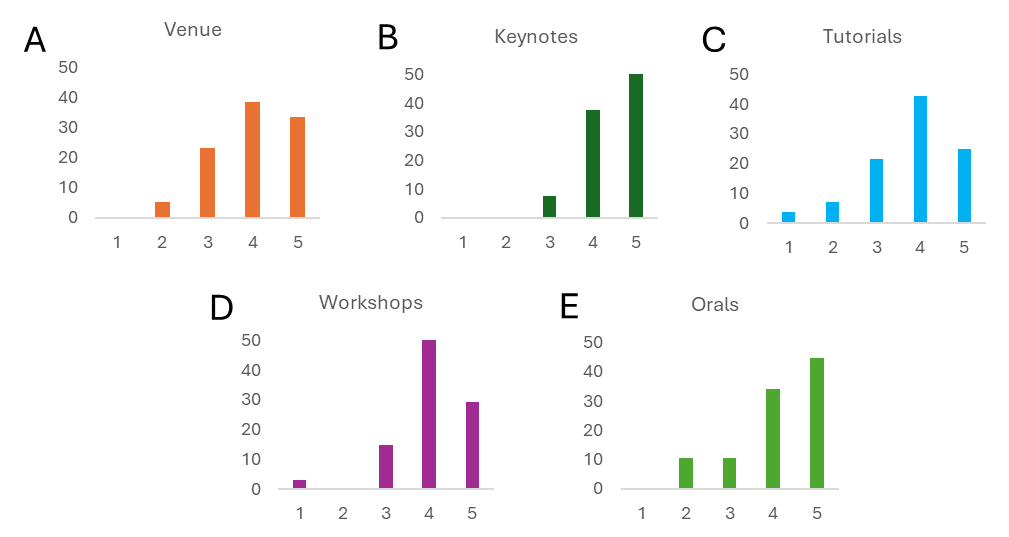
\includegraphics[width=\textwidth]{images/cns2024-feedback-form-summary}
  \caption{Summary of participant feedback, CNS*2024}%
  \label{fig:cns2024-summary}
\end{figure}


\clearpage

\section*{CNS*2025 Florence}%
\sectionauthor{??}
\lipsum[1-3]

\clearpage
\section*{Initiatives: Software Working Group}%
\sectionauthor{Marcel Stimberg \\
Ankur Sinha}
\lipsum[1-3]

\clearpage
\section*{Initiatives: Mentoring Program Updates}%
\sectionauthor{Eirini}
\begin{wrapfigure}{l}{0.2\textwidth}
  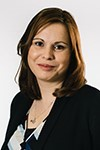
\includegraphics[width=0.2\textwidth]{images/Mavritsaki}
\end{wrapfigure}

\lipsum[1-3]

\clearpage
\section*{Elections}%
%{\large Thomas Nowotny, Professor of Informatics, University of Sussex, UK\\}
\rule{\textwidth}{0.4pt}
\lipsum[1-3]

\clearpage
% break into separate file, since we expect this to be along section
\section*{OCNS:\ Member Updates: Scientific Items}%
\sectionauthor{Updates of scientific interest from OCNS members}

\noindent{}The name of the OCNS member that submitted the entry is highlighted in \textbf{bold}.

\nocite{*}
\printbibliography[heading=none]

\clearpage
% break into separate file, since we expect this to be along section
\section*{OCNS: Member Updates: Community Development}%
\sectionauthor{Updates related to community development from OCNS members}

\begin{itemize}
    \item \textbf{The Capo Caccia Worskhops toward Neuromorphic Intelligence}

        Submitted by: Mihai A Petrovici

        \url{https://capocaccia.cc/en/event/ccnw24/landing-page/}

        The goal of the CCNW workshops is to promote the neuromorphic approach to designing technologies, establish an international community, and to encourage collaboration amongst small groups, in order to achieve the kind of technical advances which could only otherwise happen in well-funded industrial labs.

        The CCNW has an open format, whose intention is to encourage creativity and exploration of ideas and projects in a relaxed and intellectually open environment. Although there is a skeleton program that sets a default route through the two weeks, ad hoc deviations from or elaborations of this basic program are encouraged. Discussion groups and projects arise dynamically. There are no formal lectures. Instead, the morning consist of two 1.5 hr discussion sessions in which a few discussants will make short contributions to the topics in order to ignite more general interaction. Although the sessions of the skeleton program have assigned moderators and discussants, these persons should also be seen as defaults. Whiteboards and overhead tablets are available for drawings. Formal presentations with prepared media (such as Powerpoint slides) are strictly forbidden. The daily program includes a late afternoon sports break, and happy hour.


    \item \textbf{The Lu.i educational neurons}

        Submitted by: Mihai A Petrovici

        \url{https://physiologie.unibe.ch/~petrovici/group/lui.aspx}

        With an increasing presence of science throughout all parts of society, there is a rising expectation for researchers to effectively communicate their work and, equally, for teachers to discuss contemporary findings in their classrooms. While the community can resort to an established set of teaching aids for the fundamental concepts of most natural sciences, there is a need for similarly illustrative experiments and demonstrators in neuroscience. We therefore introduce Lu.i: a parametrizable electronic implementation of the leaky-integrate-and-fire neuron model in an engaging form factor. These palm-sized neurons can be used to visualize and experience the dynamics of individual cells and small spiking neural networks. When stimulated with real or simulated sensory input, Lu.i demonstrates brain-inspired information processing in the hands of a student. As such, it is actively used at workshops, in classrooms, and for science communication. As a versatile tool for teaching and outreach, Lu.i nurtures the comprehension of neuroscience research and neuromorphic engineering among future generations of scientists and in the general public.

    \item \textbf{Neuroscience Gateway (NSG)}

        Submitted by: Amitava Majumdar

        \url{https://www.nsgportal.org}

        NSG project provides free and open access to supercomputing resources. NSG enables modeling, simulation and data processing (e.g. EEG, MEG, fMRI etc.) research in neuroscience by lowering the administrative and technical barriers that currently make it difficult for investigators to use large scale computing resources. It provides access to popular neuroscience tools, pipelines, data processing software and libraries.


\end{itemize}
\newpage
\begin{itemize}
    \item \textbf{Advanced Scientific Programming in Python Summer School}

        Submitted by: Anathanasia \enquote{Nassi} Papoutsi

        \url{https://aspp.school}

        The Institute of Molecular Biology and Biotechnology of the Foundation for Research and Technology Hellas (IMBB-FORTH) at Heraklion, Crete, Greece hosted the 16th Advanced Scientific Programming in Python Summer School from August 26th to August 31st, 2024. The Summer School, kindly funded by Tubingen AI Center, was attended by 30 participants from all over the world. The interactive lectures, pair programming sessions, and coding tournaments made for an unforgettable experience. A huge thanks to our amazing participants, faculty, and organizers for bringing so much energy and enthusiasm!

\end{itemize}


\clearpage
\section*{Messages from our Sponsors}%
\sectionauthor{Short messages from OCNS sponsors}
\subsection*{Metacell}%
\begin{displayquote}
  Thank you to OCNS for hosting an excellent annual meeting, and to everyone who connected with MetaCell, attended our presentation and joined our event.
  It was great catching up with friends and partners in Natal, and we were proud sponsors of the meeting!

  If you're interested in new ways to standardize, visualize, share, and build your computational models, please visit \url{metacell.us} and get in touch with our team.
\end{displayquote}

\clearpage
\section*{INCF Updates}%
\sectionauthor{Helena/Matthew}
\lipsum[1-3]

\end{document}

